%%%%%%%%%%%%%%%%%%%%%%%%%%%%%%%%%%%%%%%%%%%%%%%%%%%%%%%%
%%%%%%%%%%%%%%%%%%%%%%%%%%%%%%%%%%%%%%%%%%%%%%%%%%%%%%%%
\section{Time Series Analysis}
\label{additional:time_series}
% https://www.youtube.com/playlist?list=PLvcbYUQ5t0UHOLnBzl46_Q6QKtFgfMGc3

Time series analysis is the study of time-dependent data such as price over time.
Similar to regression models we aim to fit a model
to the data in order to make future predictions.
However, instead of interpolating within a range of previously observed data points,
time series aims to extrapolate from our current data into the future,
as we are not interested in making predictions about past dates.
As we extrapolate further and further away from observed data
the uncertainty of our predictions will naturally grow,
making time series a harder problem to address than normal regression.
There are a variety of potential models to choose from,
each with their own assumptions and use cases.
The problem can be attacked from two general directions,
frequency-domain methods and time-domain methods,
but we shall focus primarily on the time-domain here.
The \texttt{statsmodels} \href{https://www.statsmodels.org}{python module}
is very useful for implementing these modeling methods,
which will be referenced as appropriate.

\subsubsection{Lag Notation}
\label{additional:time_series:L}

When working with time series data we often index time steps as $t$, $t-1$, $t-2$,\,\ldots\,
where $t$ is the current time.
The value of the variable in question, price, quantity, \etc,
at time $t$ is then $y_{t}$, with $y_{t-1}$, $y_{t-2}$,\,\ldots\, at subsequent times.
Instead of writing subscripts, sometimes it is more convenient
to switch to a polynomial based notation using
the lag operator $L$, also known as the backshift operator $B$ in some texts:

\begin{equation}\label{eq:time_series:L}
L y_{t} = y_{t-1},\quad L^{2} y_{t} = y_{t-2},\,\ldots \quad L^{k} y_{t} = y_{t-k}.
\end{equation}

%%%%%%%%%%%%%%%%%%%%%%%%%%%%%%%%%%%%%%%%%%%%%%%%%%%%%%%%
\subsection{Correlation in Time Series}
\label{additional:time_series:correlation}

In time series analysis $y_{t}$ can depend, to varying degree,
on the previous values $L^{k} y_{t},\, \forall k$.
There is a direct component to this dependence,
$y_{t} \sim f\left(y_{t-1}\right)$,
but also an indirect or recursive component,
$y_{t} \sim f\left(y_{t-1}\right) \sim f\left(g\left(y_{t-2}\right)\right)$.

\subsubsection{Auto-Correlation Function (ACF)}
\label{additional:time_series:ACF}

Neglecting the multiple components of the correlation of $y_{t}$ with prior times,
we can commute the overall auto-correlation function (ACF) of $y_{t}$
with itself at some amount of lag $k$ as

\begin{equation}\label{eq:time_series:ACF}
\text{ACF}\left(y,k\right) = \corr{y_{t}}{y_{t-k}},
\end{equation}

\noindent using the regular Pearson correlation coefficient \cref{eq:stats:corr}.
The auto-correlation shows the total correlation and is simple to compute,
but mixes the direct and indirect effects of prior values together.

\subsubsection{Partial Auto-Correlation Function (PACF)}
\label{additional:time_series:PACF}

In contrast, partial auto-correlation function
aims to isolate the direct influence of $y_{t-k}$ on $y_{t}$ for some lag $k$.
We can get at this component by fitting $y_{t}$ as a linear function of $L^{n} y_{t}$,

\begin{equation}\label{eq:time_series:PACF}
y_{t} = \sum_{i=1}^{k} \phi_{k,i}\, y_{t-i} + \epsilon_{k},
\end{equation}

\noindent and identifying $\text{PACF}\left(y,k\right) = \phi_{k,k}$
as the partial auto-correlation function for $k$.
Note that for each $k$, we need to do a new fit of \cref{eq:time_series:PACF},
and after fitting should check that $\phi_{k,k}$ is statistically significant,
\ie we reject $H_{0}$ that $\phi_{k,k}=0$, by looking at the coefficient's confidence interval from the fit.
We can generate plots of ACF and PACF vs $k$ to explore a time series
with the \texttt{plot\_acf} and \texttt{plot\_pacf}
\href{https://www.statsmodels.org/stable/graphics.html\#time-series-plots}{functions}.

%%%%%%%%%%%%%%%%%%%%%%%%%%%%%%%%%%%%%%%%%%%%%%%%%%%%%%%%
\subsection{Stationarity}
\label{additional:time_series:stationarity}

Stationarity is an important assumption for many parametric time series models,
which combines three properties:

\begin{enumerate}[noitemsep]
  \item The mean $\expval{y}$ of the time series is constant, \ie the average is not moving.\label{item:time_series:stationarity:constant_mean}
  \item The variance $\variance{y}$ of the time series is constant.\label{item:time_series:stationarity:constant_var}
  \item The time series does not exhibit seasonality, \ie no periodic fluctuations in $y\left(t\right)$.\label{item:time_series:stationarity:seasonality}
\end{enumerate}

If the mean or variance is growing with time
we can look at the first difference, $\widetilde{y}_{t} = y_{t} - y_{t-1}$,
and see if the time series of $\widetilde{y}_{t}$ is stationary,
see \cref{additional:time_series:I} for more.
Similarly, we can try to remove seasonality
by subtracting a deterministic time-dependent function $f\left(t\right)$
or by using the SARIMA model of \cref{additional:time_series:SARIMA}.
We can also try normalizing with a $Z$-score to address a changing mean or variance;
subtracting or dividing as needed to make the series more stationary.
This even works with seasonality if we subtract the mean value per medium-sized time unit, \eg month, quarter, \etc.
When cleaning the data in this way,
we will need to invert any preprocessing steps
while making predictions to return to the original units.

Simply looking at the graph of a time series can give us
a good intuition on if it is stationary or not.
However, we can formally test for stationarity
with the augmented Dickey--Fuller test (ADF) of \cref{additional:time_series:ADF}.

%%%%%%%%%%%%%%%%%%%%%%%%%%%%%%%%%%%%%%%%%%%%%%%%%%%%%%%%
\subsection{White Noise}
\label{additional:time_series:white_noise}

In the context of time series analysis, white noise is random fluctuations which
have mean zero, $\expval{y} = 0$,
constant variance with respect to time, $\partial_{t} \variance{y} = 0$,
and no correlation between lags, $\corr{y_{t}}{y_{t-k}} = 0,\,\, \forall k$.
Ideally after fitting a time series, we will capture all of the signal
in the model and the resulting error term $\epsilon$ will only contain white noise.
We can test for white noise by looking at the moving average and ACF plot,
or more formally with the Ljung--Box test of \cref{additional:time_series:ljung_box}.

%%%%%%%%%%%%%%%%%%%%%%%%%%%%%%%%%%%%%%%%%%%%%%%%%%%%%%%%
\subsection{Autoregressive (AR) Models}
\label{additional:time_series:AR}
Building on the PACF, we can construct an autoregressive (AR) model $\text{AR}\left(p\right)$
from multiple lag components of the time series:

\begin{equation}\label{eq:time_series:AR}
\hat{y}_{t} = \phi_{0} + \sum_{i=1}^{p} \phi_{i}\, y_{t-i} + \epsilon_{t}.
\end{equation}

Note that we should look at the PACF plot before fitting \cref{eq:time_series:AR}
to determine which lags to include,
\ie set $p$ and decide which lags to skip\footnote{It may not be possible
to specify individual lags to include in some software packages,
but excluding non-significant coefficients and reducing model complexity
is still a good idea if possible.} by setting $\phi_{i} = 0$.

%%%%%%%%%%%%%%%%%%%%%%%%%%%%%%%%%%%%%%%%%%%%%%%%%%%%%%%%
\subsection{Moving Average (MA) Models}
\label{additional:time_series:MA}

Instead of looking at the auto-correlation $y_{y-i}$,
we can also build a time series model around
correcting for prior errors in the prediction,
\ie fitting to the moving average (MA).
The $\text{MA}\left(q\right)$ model
is then:

\begin{subequations}\label{eq:time_series:MA}
\begin{align}
\hat{y}_{t} &= \theta_{0} + \sum_{i=1}^{q} \theta_{i}\, \epsilon_{t-i} + \epsilon_{t}, \label{eq:time_series:MA_y} \\
\epsilon_{t-1} &= y_{t-1} - \hat{y}_{t-1}. \label{eq:time_series:MA_epsilon}
\end{align}
\end{subequations}

Note that a $\text{MA}\left(q\right)$ model will fluctuate around the initial average $\theta_{0}$,
and can only predict $q$ steps into the future before constantly returning $\theta_{0}$.
We can select $q$ by looking at the ACF plot
and identifying the last non-zero lag.

%%%%%%%%%%%%%%%%%%%%%%%%%%%%%%%%%%%%%%%%%%%%%%%%%%%%%%%%
\subsection{Invertibility of Time Series}
\label{additional:time_series:invert}
% https://youtu.be/QU_VNu3rJKY
% https://youtu.be/q0vz7dGlZL0

One interesting property of AR and MA time series models is their invertibility:

\begin{subequations}\label{eq:time_series:invert}
\begin{align}
\text{MA}\left(1\right) &= \text{AR}\left(\infty\right), \label{eq:time_series:invert:MA_1} \\
\text{AR}\left(1\right) &= \text{MA}\left(\infty\right). \label{eq:time_series:invert:AR_1}
\end{align}
\end{subequations}

For a proof of \cref{eq:time_series:invert:MA_1}, see \cref{eq:time_series:invert_proof}.
Letting $\theta = \phi < 0$ for convenience and
assuming\footnote{Here we are assuming the time series is stationary, \ie no unit roots $\abs{\phi} < 1$.} $\abs{\phi} < 1$
we can construct the time series $C_{t}$,

\begin{subequations}\label{eq:time_series:invert_proof}
\begin{align}
C_{t} \equiv \text{MA}\left(1\right) - \theta_{0} &= -\phi\, \epsilon_{t-1} + \epsilon_{t} = \left(1 - \phi L \right) \epsilon_{t}, \label{eq:time_series:invert_proof:a} \\
\implies \epsilon_{t} &= \frac{C_{t}}{1 - \phi L}, \label{eq:time_series:invert_proof:b} \\
&= \left(\,\sum_{i=0}^{\infty} \phi^{i} L^{i} \right) C_{t} = \sum_{i=0}^{\infty} \phi^{i} C_{t-i}, \label{eq:time_series:invert_proof:c} \\
\implies C_{t} &= \sum_{i=1}^{\infty} -\phi^{i} C_{t-i} + \epsilon_{t} = \text{AR}\left(\infty\right) - \phi_{0}, \label{eq:time_series:invert_proof:d}
\end{align}
\end{subequations}

\noindent where in \cref{eq:time_series:invert_proof:c} we have used
the sum of a geometric series \cref{eq:additional:misc:math:geometric}.
The proof of \cref{eq:time_series:invert:AR_1} is similar and also relies on the geometric series.
Essentially we are making the recursive nature of these time series explicit and using it to transform from one to the other.
The $\text{AR}\left(\infty\right)$ expansion of $\text{MA}\left(1\right)$
is particularly useful as it is possible in practice to truncate the series at $\order{\phi^{\,p}}$
where $\phi^{\,p} \approx 0$ and represent $\text{MA}\left(1\right)$ as
a pure function of the time series itself, \ie without recursion.

%%%%%%%%%%%%%%%%%%%%%%%%%%%%%%%%%%%%%%%%%%%%%%%%%%%%%%%%
\subsection{ARMA Model}
\label{additional:time_series:ARMA}

While we can represent AR $\Leftrightarrow$ MA with infinite series,
it is more practical to include both in one model with a finite number of terms.
The $\text{ARMA}\left(p,q\right)$ model is a simple combination of
both approaches:

\begin{equation}\label{eq:time_series:ARMA}
\hat{y}_{t} = \mu_{0} + \sum_{i=1}^{p} \phi_{i}\, y_{t-i} + \sum_{i=1}^{q} \theta_{i}\, \epsilon_{t-i} + \epsilon_{t}.
\end{equation}

Using lag notation we can write \cref{eq:time_series:ARMA} more
compactly\footnote{We drop
the constant intercept terms for convenience, as do many other sources.
However a constant term can still be included if desired,
or we can construct $\widetilde{y}_{t} = y_{t} - \mu_{0}$ with $\expval{\widetilde{y}_{t}} = 0$.}\footnote{If we set
$\phi_{0}=-1$, $\theta_{0} = 1$ and start the sums at $i=0$
we can simplify \cref{eq:time_series:ARMA_lag} even further.} as

\begin{subequations}\label{eq:time_series:ARMA_lag}
\begin{align}
\phi\left(L,p\right) y_{t} &= \theta\left(L,q\right) \epsilon_{t}, \label{eq:time_series:ARMA_lag:def} \\
\phi\left(L,p\right) &= 1 - \sum_{i=1}^{p} \phi_{i}\, L^{i}, \label{eq:time_series:ARMA_lag:phi} \\
\theta\left(L,q\right) &= 1 + \sum_{i=1}^{q} \theta_{i}\, L^{i}, \label{eq:time_series:ARMA_lag:theta}
\end{align}
\end{subequations}

\noindent where \cref{eq:time_series:ARMA_lag:phi,eq:time_series:ARMA_lag:theta} are polynomials of the lag operator $L$.
To avoid parameter redundancy, \ie multiple $\phi$, $\theta$ coefficients for $\order{L^{n}}$,
we require the polynomials $\phi\left(L,p\right)$ and $\theta\left(L,q\right)$ to not share any common factors.

%%%%%%%%%%%%%%%%%%%%%%%%%%%%%%%%%%%%%%%%%%%%%%%%%%%%%%%%
\subsection{Integrated (I) Models}
\label{additional:time_series:I}

The previous models have worked well for stationary time series with constant means,
however we may wish to model a quantity with a mean that linearly changes over time.
One method of incorporating this behavior in a time series model is by
recursively taking the difference $d$ times between lags of the original time series $y_{t}$
to construct a new time series $\widetilde{y}_{t}$ \cref{eq:time_series:I:forward}.
With the appropriate choice of $d$, typically $d \leq 2$,
$\widetilde{y}_{t}$ should have a constant mean,
allowing other models to be subsequently used.
This process is known as the integrated model $\text{I}\left(d\right)$,
though the name is misleading as what we are really doing is differentiating $y$ to find a constant slope, curvature, \etc.
Note, when making predictions we will need to
transform back to the original $y_{t}$ \cref{eq:time_series:I:backward1,eq:time_series:I:backward2},
at the cost of $d$ initial data points where no predictions can be made.

\begin{subequations}\label{eq:time_series:I}
\begin{align}
\widetilde{y}_{t} &= \left(1-L\right)^{d} y_{t}, \label{eq:time_series:I:forward} \\
y_{t} &= \widetilde{y}_{t} + y_{t-1},\,\, \text{where}\,\, d=1, \label{eq:time_series:I:backward1} \\
y_{t} &= \widetilde{y}_{t} + 2 y_{t-1} - y_{t-2},\,\, \text{where}\,\, d=2. \label{eq:time_series:I:backward2}
\end{align}
\end{subequations}

%%%%%%%%%%%%%%%%%%%%%%%%%%%%%%%%%%%%%%%%%%%%%%%%%%%%%%%%
\subsection{ARIMA Model}
\label{additional:time_series:ARIMA}

Putting everything together, we can construct the $\text{ARIMA}\left(p,d,q\right)$ model
by including \cref{eq:time_series:I:forward} in \cref{eq:time_series:ARMA_lag}:

\begin{equation}\label{eq:time_series:ARIMA}
\phi\left(L,p\right) \left(1-L\right)^{d} y_{t} = \theta\left(L,q\right) \epsilon_{t}.
\end{equation}

\subsubsection{ARIMA Model Example}
\label{additional:time_series:ARIMA:ex}

% TODO include example plots of y_{t}, PACF, ACF, predictions, and residuals; and link to the example notebook

%%%%%%%%%%%%%%%%%%%%%%%%%%%%%%%%%%%%%%%%%%%%%%%%%%%%%%%%
\subsection{Seasonal ARIMA Model (SARIMA)}
\label{additional:time_series:SARIMA}

Extending the ideas of the integrated model from \cref{additional:time_series:I},
we can attempt to control for seasonality by
taking lags across $m$ time steps at once, \ie using $L^{m}$ in place of $L$.
For example, if $m=12$ corresponds to 1 year,
we will be doing the normal extrapolation of ARIMA on $y_{t-1-1\,\text{Year}}$ instead of $y_{t-1}$,
thereby canceling out any yearly periodic trends.
The resulting $\text{SARIMA}\left(p,d,q\right)\left(P,D,Q\right)_{m}$ model
has the normal $\text{ARIMA}\left(p,d,q\right)$ model components,
plus an additional set\footnote{Details around
coefficient conditions and parameter redundancy are omitted for brevity.} of uppercase parameters
controlling a $L^{m}$ based ARIMA model:

\begin{equation}\label{eq:time_series:SARMA}
\phi\left(L,p\right) \Phi\left(L^{m},P\right) \left(1-L\right)^{d} \left(1-L^{m}\right)^{D} y_{t} = \theta\left(L,q\right) \theta\left(L^{m},q\right) \epsilon_{t}.
\end{equation}

The $\text{SARIMA}\left(p,d,q\right)\left(P,D,Q\right)_{m}$ family of models
is available via the \texttt{ARIMA}
\href{https://www.statsmodels.org/stable/generated/statsmodels.tsa.arima.model.ARIMA.html}{class},
with a wide variety of attributes and methods
enabling us to implement all of the above time series models.
Computationally, \texttt{ARIMA} preforms fits via maximum likelihood estimation (MLE),
but AR models can also be fit with ordinary least squares (OLS).

%%%%%%%%%%%%%%%%%%%%%%%%%%%%%%%%%%%%%%%%%%%%%%%%%%%%%%%%
\subsection{ARMA Model with Exogenous Inputs (ARMAX)}
\label{additional:time_series:ARMAX}

The $\text{ARMAX}\left(p,q,b\right)$ model
extends ARMA by incorporating exogenous (X) inputs
via another known time series $d_{t}$:

\begin{equation}\label{eq:time_series:ARMAX}
\hat{y}_{t} = \mu_{0} + \sum_{i=1}^{p} \phi_{i}\, y_{t-i} + \sum_{i=1}^{q} \theta_{i}\, \epsilon_{t-i} + \sum_{i=1}^{b} \eta_{i}\, d_{t-i} + \epsilon_{t}.
\end{equation}

We can think of the $d_{t}$ time series like the driving force of a driven harmonic oscillator.
In practice, ARMAX usually is implemented as ARMA on
a transformed $y_{t}$ which takes into account different lags of $d_{t}$,
so careful interpretation of a given software package's outputs and documentation is required.
The \texttt{ARIMA}
\href{https://www.statsmodels.org/stable/generated/statsmodels.tsa.arima.model.ARIMA.html}{class}
can incorporate an exogenous time series,
as well as deterministic polynomials of $t$,
\ie the $f\left(t\right)$ mentioned in \cref{additional:time_series:stationarity}.

%%%%%%%%%%%%%%%%%%%%%%%%%%%%%%%%%%%%%%%%%%%%%%%%%%%%%%%%
\subsection{Other Models (VAR, ARCH, GARCH, Bayesian Approaches)}
\label{additional:time_series:other_models}

In addition to the SARIMAX family of models detailed above,
there are a few other useful time series models to note here.
The vector autoregression (VAR) model is a matrix based
generalization of $\text{AR}\left(p\right)$ to multiple dimensions.
See the \texttt{vector\_ar}
\href{https://www.statsmodels.org/stable/generated/statsmodels.tsa.vector_ar.var_model.VAR.html}{class} for more.

The autoregressive conditional heteroskedasticity (ARCH) and generalized ARCH (GARCH) models,
popular in finance, are appropriate when the underlying time series
exhibits periodic episodes of increased variance\footnote{Conditional heteroskedasticity meaning periodically differing variances.}.
These models predict the volatility $\sigma_{t}^{2}$ as a function of
the prior errors $\epsilon_{t-1}$ and variances $\sigma_{t-1}^{2}$
which allow them to cope with ``bursty'' periods of increased volatility.
See the \texttt{arch}
\href{https://arch.readthedocs.io/en/stable/univariate/introduction.html}{package}
for one implementation.

We can also look at time series analysis within a Bayesian framework;
assuming prior distributions for the model parameters $\bm{\beta}$
then updating based on the observed data,
thereby producing distributions of our predictions and parameters instead of only MLE point estimates.
The \texttt{PyMC3} \href{https://docs.pymc.io/en/v3/}{module}
has \href{https://docs.pymc.io/en/v3/api/distributions/timeseries.html}{timeseries functions}
for implementing this approach, including AR and GARCH models.

%%%%%%%%%%%%%%%%%%%%%%%%%%%%%%%%%%%%%%%%%%%%%%%%%%%%%%%%
\subsection{Evaluating Time Series Models}
\label{additional:time_series:eval}

Like other machine learning problems, we must split our data into train and test sets
when fitting and evaluating time series models.
As we are extrapolating we use the first
$\approx \SI{70}{\percent}$ of the data by time for the training set,
and the reminding $\approx \SI{30}{\percent}$ for the test set,
instead of randomly splitting the data as is done for interpolative models.
To improve on this approach even further, we can use
rolling forecast origin techniques to evaluate the model.
In short, we use the first $k$ data points to train the model,
evaluate it on the next $k + l$ data points, increment $k$ and reiterate.
Performance metrics can then be averaged across the iterations.
In this way the model's near term predictions at each iteration are as accurate as possible,
as if time had continued and we received more data,
giving a better estimate of the predictive performance in practice.
There are a few different methods for how to exactly roll the origin,
see \cref{fig:rolling_forecast_origin} for details.

\begin{figure}
\centering
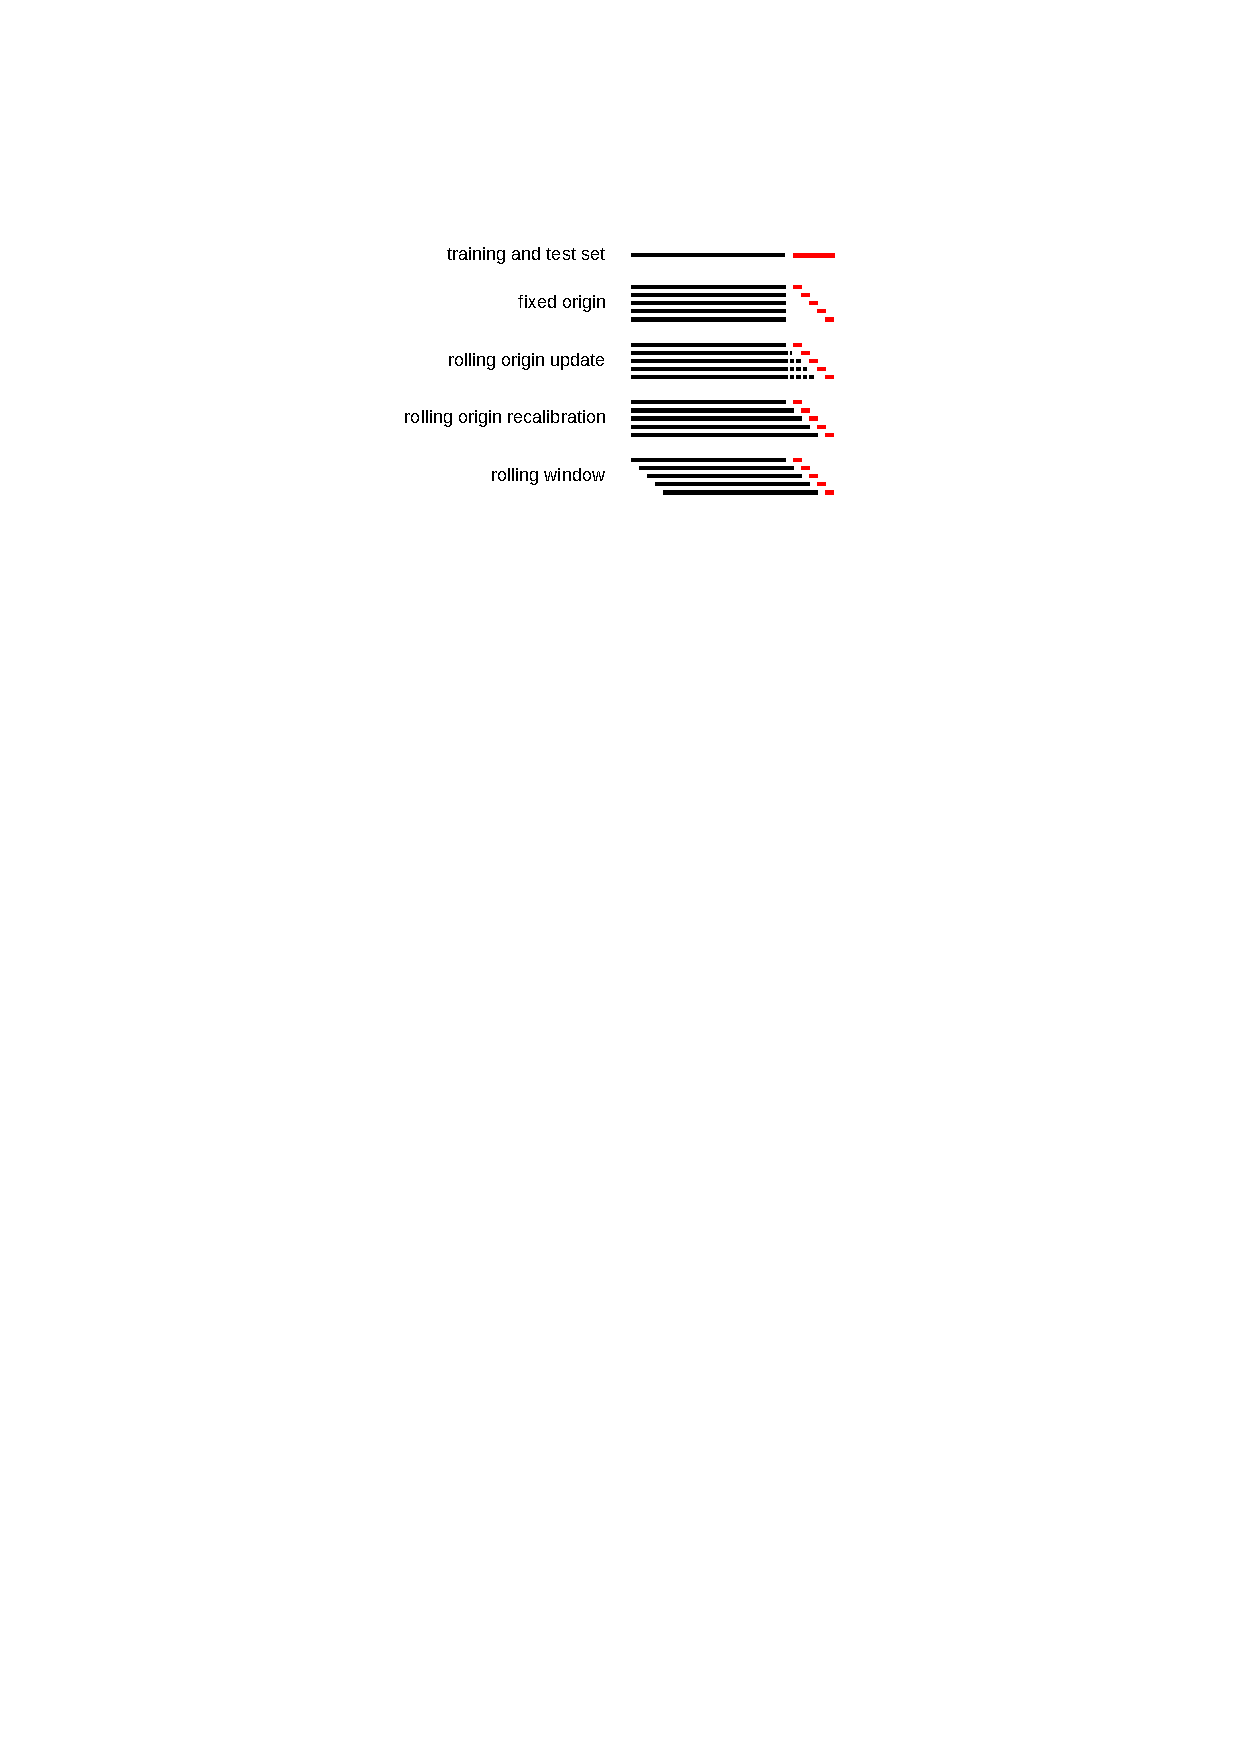
\includegraphics[width=0.6\textwidth]{figures/stats/rolling_forecast_origin}
\caption{
Illustration of multiple test train split methods for time series models \cite{bergmeir_dissertation}.
Note that $t$ is increasing along the $x$-axis.
In the fixed origin method, we do not do any retraining and the prediction quality
can be expected to drop as we go further into the future.
In the rolling origin update method, we do not retrain the model parameters $\bm{\beta}$
with each iteration, but do update the $y_{i}$ lags.
In the rolling origin recalibration method we fully retrain the model on each iteration.
Lastly, in the rolling window method we remove data from the beginning of the training period
as we iterate to keep the training set a constant size.
This can help with some statistical interpretations of the model,
but also helps when working with slowly changing non-stationary data.
}
\label{fig:rolling_forecast_origin}
\end{figure}

Regardless of the test train split method, we can get a sense of the model's performance
qualitatively by looking at residual plots of $y_{t} - \hat{y}_{t}$.
The residuals will show any remaining systematic trends that the model did not learn,
as ideally they would be white noise.
Quantitatively, we can test
if the residuals are white noise with the Ljung--Box test of \cref{additional:time_series:ljung_box},
as well as can compute the
root mean squared error\footnote{Also known as the root mean squared deviation (RMSD).} (RMSE)
and mean absolute percent error (MAPE)
between the predictions and observed values:

\begin{subequations}\label{eq:time_series:RMSE_MAPE}
\begin{align}
\text{RMSE}\left(\hat{y}\right) &= \sqrt{\expval{\left(y - \hat{y}\right)^{2}}} = \sqrt{\frac{1}{n}\sum_{t=1}^{n} \left(y_{t} - \hat{y}_{t}\right)^{2}}, \label{eq:time_series:RMSE} \\
\text{MAPE}\left(\hat{y}\right) &= \frac{\SI{100}{\percent}}{n} \sum_{t=1}^{n} \abs{\frac{y_{t} - \hat{y}_{t}}{y_{t}}}\,. \label{eq:time_series:MAPE}
\end{align}
\end{subequations}

\subsubsection{AIC, BIC}
\label{additional:time_series:AIC_BIC}

% TODO
% https://youtu.be/McEN54l3EPU

%%%%%%%%%%%%%%%%%%%%%%%%%%%%%%%%%%%%%%%%%%%%%%%%%%%%%%%%
\subsection{Box--Jenkins Method (Expanded)}
\label{additional:time_series:box_jenkins}

The Box--Jenkins method, popularized in their book \cite{boxjen76},
is a recipe for fitting an ARMA-based model to a given time series $y_{t}$.
The steps have been expanded here to make the entire process
for working with time series data more explicit:

\begin{enumerate}[noitemsep]
  \item Do any necessary pre-cleaning of $y_{t}$ to normalize the data.\label{item:time_series:box_jenkins:cleaning0}
  \begin{enumerate}[noitemsep]
    \item $Z$-score normalization, deterministic transforms $f\left(t\right)$, \etc.\label{item:time_series:box_jenkins:cleaning0:detail}
    \item Also, split the training and test sets.\label{item:time_series:box_jenkins:cleaning0:train_test_split}
  \end{enumerate}
  \item Check the stationarity and seasonality of the cleaned $y_{t}$.\label{item:time_series:box_jenkins:assumptions}
  \begin{enumerate}[noitemsep]
    \item Look at $y_{t}$ and the MA plot for obvious problems.\label{item:time_series:box_jenkins:assumptions:eye}
    \item Use the augmented Dickey--Fuller test (ADF) for stationary.\label{item:time_series:box_jenkins:assumptions:ADF}
    \item Correct any remaining problems with a ARIMA, $1 \leq d$, or SARIMA model.\label{item:time_series:box_jenkins:assumptions:cleaning1}
  \end{enumerate}
  \item Select the appropriate ARMA model, \ie choose $p$ and $q$.\label{item:time_series:box_jenkins:order}
  \begin{enumerate}[noitemsep]
    \item The PACF plot gives clues to the $\text{AR}\left(p\right)$ order.\label{item:time_series:box_jenkins:order:PACF}
    \item The ACF plot gives clues to the $\text{MA}\left(q\right)$ order.\label{item:time_series:box_jenkins:order:ACF}
  \end{enumerate}
  \item Fit the chosen model.\label{item:time_series:box_jenkins:fit}
  \item Verify the fitted model by checking the residuals. Return to \cref{item:time_series:box_jenkins:cleaning0} if needed.\label{item:time_series:box_jenkins:verify}
  \begin{enumerate}[noitemsep]
    \item Use the Ljung--Box test for white noise on the residuals.\label{item:time_series:box_jenkins:verify:Ljung_Box}
    \item Measure performance with RMSE and MAPE.\label{item:time_series:box_jenkins:verify:RMSE_MAPE}
  \end{enumerate}
  \item Invert any cleaning steps to return to the original units of $y_{t}$ for predictions.\label{item:time_series:box_jenkins:invert}
\end{enumerate}

In \cref{item:time_series:box_jenkins:order} a simple approach is to
go out to the last significant non-zero order of $p$ ($q$) in the PACF (ACF) plot.
However, interpreting the PACF and ACF plots is a developed skill
and there are many different pieces of advice
available\footnote{See
\href{https://people.duke.edu/~rnau/411arim3.htm}{here}
and the Box--Jenkins method
\href{https://en.wikipedia.org/wiki/Box\%E2\%80\%93Jenkins\_method\#Autocorrelation\_and\_partial\_autocorrelation\_plots}{wiki page}
for just two examples.}.

%%%%%%%%%%%%%%%%%%%%%%%%%%%%%%%%%%%%%%%%%%%%%%%%%%%%%%%%
\subsection{Unit Roots}
\label{additional:time_series:unit_root}

% TODO
% https://youtu.be/ugOvehrTRRw

%%%%%%%%%%%%%%%%%%%%%%%%%%%%%%%%%%%%%%%%%%%%%%%%%%%%%%%%
\subsection{Augmented Dickey--Fuller (ADF) Test for Stationarity}
\label{additional:time_series:ADF}

The augmented\footnote{The ADF is an extension of the normal Dickey--Fuller test where $p = 1$.} Dickey--Fuller (ADF) test
is a hypothesis tests for the stationarity of a time series.
We begin by assuming the time series for $y$ is a $\text{AR}\left(p\right)$ model \cref{eq:time_series:AR}
and construct the difference:

\begin{subequations}\label{eq:time_series:ADF}
\begin{align}
\Delta y_{t} &= y_{t} - y_{t-1} = \phi_{0} + \delta y_{t-1} + \sum_{i=2}^{p} \phi_{i}\, y_{t-i} + \epsilon_{t}, \label{eq:time_series:ADF:Delta_y} \\
\delta &= \phi_{1} - 1. \label{eq:time_series:ADF:delta}
\end{align}
\end{subequations}

Now we test $H_{0}$ that $0 \leq \delta$ and the time series is
non-stationary\footnote{As $\delta = 0 \implies \phi_{1} = 1$, \ie the time series has a unit root and is non-stationary.}
vs the alternative hypothesis $H_{a}$ that $\delta < 0$, \ie time series is stationary.
We fit the data and then perform the hypothesis testing with test statistic
$t_{\hat{\delta}} = \hat{\delta} / \text{Standard Error}\left(\hat{\delta}\right)$
by comparing to the Dickey--Fuller distribution\footnote{We can not use the standard $t$-distribution as $y_{t-1}$ is still assumed to be non-stationary under $H_{0}$.}.
If we can reject $H_{0}$ we therefore have shown that $y_{t}$ is stationary.
Note we can further extend the ADF test by replacing the constant $\phi_{0}$
with a deterministic, quadratic, time trend $\phi_{0} + a_{1} t + a_{2} t^{2}$.
The ADF test is available via the \texttt{adfuller}
\href{https://www.statsmodels.org/stable/generated/statsmodels.tsa.stattools.adfuller.html}{function}.

%%%%%%%%%%%%%%%%%%%%%%%%%%%%%%%%%%%%%%%%%%%%%%%%%%%%%%%%
\subsection{Ljung--Box Test for White Noise}
\label{additional:time_series:ljung_box}

The Ljung--Box test tests if a time series $y$ solely consists of white noise
by looking at multiple lags of the ACF.
The test statistic is

\begin{equation}\label{eq:time_series:ljung_box:Q}
Q = n \left(n+2\right) \sum_{i=1}^{h} \frac{\corr{y_{t}}{y_{t-i}}^{2}}{n-i}
\end{equation}

\noindent where $n$ is the sample size and $h$ is the number of lags to be tested.
Using the $\chi^{2}$-distribution with $\nu = h$ degrees of freedom we find the critical $Q_{c}$
and reject $H_{0}$, the data is white noise, if $Q_{c} < Q$.
If we fail to reject $H_{0}$, \ie $Q \leq Q_{c}$, we have shown $y$ is white noise.
Note that if we are performing the Ljung--Box test on the remainders of a fitted model, such as $\text{ARIMA}\left(p,d,q\right)$,
we must adjust the degrees of freedom accordingly, $\nu = h - p - d - q$.
The Ljung--Box test can be performed with the \texttt{acorr\_ljungbox}
\href{https://www.statsmodels.org/stable/generated/statsmodels.stats.diagnostic.acorr_ljungbox.html}{function}.

%%%%%%%%%%%%%%%%%%%%%%%%%%%%%%%%%%%%%%%%%%%%%%%%%%%%%%%%
\subsection{Anomaly Detection}
\label{additional:time_series:anomaly_detection}

% TODO
% https://youtu.be/XPwCo4cqqt0
